\section{Stationary states in the $\{\ket{x}\}$ representation}
%%
\subsection{Hermite polynomials}

\subsubsection{Definition}
Let be the Gaussian function 
\begin{align}
    F(z)=e^{-z^2}
\end{align}
The successive derivatives are 
\begin{align*}
    F'(z)=-2ze^{-z^2},\quad F''(z)=(4z^2-2)e^{-z^2},\quad\cdots,\quad F^{(n)}(z)=(-1)^nH_n(z)e^{-z^2}.
\end{align*}
If we have $F^{(n-1)}$, its differentiation will yields $F^{(n)}$ and we can obtain the above general equation:
\begin{align}
    H_n(z)=\left(2z-\frac{d}{dz}\right)H_{n-1}(z),
    \label{eq:relhermite}
\end{align}
where $H_n(z)$ is the nth-degree \bfemph{Hermite polynomial}:
\begin{align}
    \text{Hermite polynomial}\qquad\highlight{H_n(z)=(-1)^ne^{z^2}\frac{d^n}{dz^n}e^{-z^2}}.
    \label{eq:hermitepolynomial}
\end{align}
The parity of $H_n(x)$ is $(-1)^n$, and it has $n$ real zeros between which one finds those of $H_{n-1}$.
\begin{figure}[h!]
    \centering
    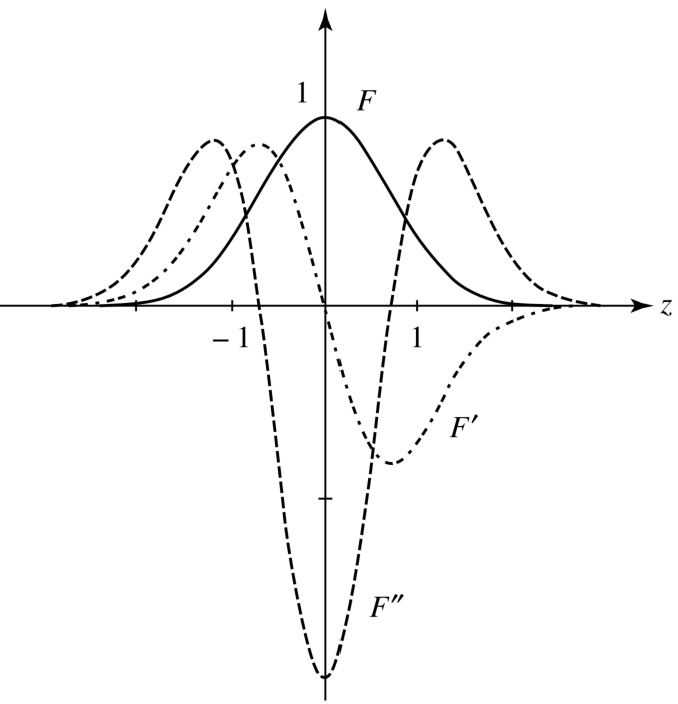
\includegraphics[width=.4\columnwidth]{PartOne/ChapterThree/gaussianandf.png}
    \caption{Shape of the Gaussian function $F(z)$ and its first and second derivatices.}
\end{figure}
%%
\subsubsection{Generating function}
Consider the function 
\begin{align*}
    F(z+\lambda)=e^{-(z+\lambda)^2}\stackrel{\text{Taylor}}{=}\sum_{n=0}^\infty\frac{\lambda^n}{n!}F^{(n)}(z)=\sum_{n=0}^\infty\frac{\lambda^n}{n!}(-1)^nH_n(z)e^{-z^2}.
\end{align*}
Multiplying this relation by $e^{z^2}$ and replacing $\lambda$ by $-\lambda$ we obtain:
\begin{align}
    \text{Generating function of Hermite polynomials}\qquad e^{z^2}F(z-\lambda)=\highlight{e^{-\lambda^2+2\lambda z}=\sum_{n=0}^\infty\frac{\lambda^n}{n!}H_n(z)}.
    \label{eq:generatingfunctionhermite}
\end{align}
The Hermite polynomials can therefore be obtained from the series expansion in $\lambda$ for the function $e^{-\lambda^2+2\lambda z}$.
%
\subsubsection{Recurrence relations; differential equation}
We can obtain other recurrence relation by using the equation \eqref{eq:generatingfunctionhermite}. For instance, differentiating equation \eqref{eq:generatingfunctionhermite} with respect to 
$z$ and using its expansion:
\begin{align}
    \frac{d}{dz}H_n(z)=2nH_{n-1}(z).
    \label{eq:diffhermite}
\end{align} 
If we differentiate with respect to $\lambda$, we get 
\begin{align}
    H_n(z)=2zH_{n-1}(z)-2(n-1)H_{n-2}(z).
\end{align}
Finally, we can obtain an ODE differentiating equation \eqref{eq:diffhermite} and using \eqref{eq:relhermite}:
\begin{align*}
    \frac{d^2}{dz^2}H_n(z)=2n\frac{d}{dz}H_{n-1}(z)=2n[2zH_{n-1}(z)-H_n(z)]=2z\frac{d}{dz}H_{n-1}(z)-2nH_n(z),
\end{align*}
Thus,
\begin{align}
    \text{ODE satisfied by Hermite polynomials}\qquad\highlight{\left[\frac{d^2}{dz^2}-2z\frac{d}{dz}+2n\right]H_n(z)=0}.
\end{align}
%%
\subsection{The eigenfunctions of the harmonic oscillator Hamiltonian}
%
\subsubsection{Generating function}

%
\subsubsection{$\varphi_n(x)$ in terms of the Hermite polynomials}
What is $\varphi(x)=\braket{x|\varphi}$?

We know that $a\ket{\varphi_0}=0\ket{\varphi_0}$, so we replace the $\{\ket{x}\}$ representation 
\begin{align*}
    \braket{x|a|\varphi_0}=\braket{x|\frac{1}{\sqrt{2}}\left(\frac{x}{\sigma}+\frac{ip\sigma}{\hbar}\right)|\varphi_0}&=0\\
    \frac{1}{\sqrt{2}}\left(\frac{x}{\sigma}+\sigma\frac{\partial}{\partial x}\right)\varphi_0(x)&=\\
    \frac{\partial\varphi_0(x)}{\partial x}&=-\frac{x}{\sigma^2}\varphi_0(x).
\end{align*}
Its solution is 
\begin{align*}
    \varphi_0(x)=ce^{-\frac{x^2}{2\sigma^2}}\stackrel{\text{normalization}}{\longrightarrow}\varphi_0(x)=\left(\frac{1}{\pi\sigma^2}\right)^{1/4}e^{-\frac{x^2}{2\sigma^2}}.
\end{align*}

The general form is the following:
\begin{align}
    \text{Excited state in $\{\ket{x}\}$}\qquad\highlight{\varphi_n(x)=
    \left(\frac{\beta^2}{\pi}\right)^{1/4}\frac{1}{\sqrt{2^nn!}}e^{-\beta^2x^2/2}H_n(\beta x)}.
\end{align}
The shape of $\varphi_n(x)$ is therefore analogous to that of the nth-order derivative of the Gaussian function $F(x)$. Moreover, $\varphi_n(x)$ is of parity 
$(-1)^n$ and posseses $n$ zeros interposed between those of $\varphi_{n+1}(x)$. Recall this is related to the increase in the average kinetic energy of the 
states $\ket{\varphi_n}$ when $n$ increases.
%
\subsubsection{Recurrence relations}
Lets write the action of $a$ and $a^\dagger$ \eqref{eq:actionofaa} in the $\{\ket{x}\}$ representation. The action of them 
in this representation is 
\begin{align}
    a\longrightarrow \frac{\beta}{\sqrt{2}}\left[x+\frac{1}{\beta^2}\frac{d}{dx}\right]\qquad a^\dagger\longrightarrow\frac{\beta}{\sqrt{2}}\left[x-\frac{1}{\beta^2}\frac{d}{dx}\right].
\end{align}
Then equation \eqref{eq:actionofaa} becomes:
\begin{align}
    \text{Action of $a,a^\dagger$ in $\{\ket{x}\}$}\qquad\highlight{
        \begin{array}{l}
            \dfrac{\beta}{\sqrt{2}}\left[x+\dfrac{1}{\beta^2}\dfrac{d}{dx}\right]\varphi_n(x)=\sqrt{n}\varphi_{n-1}(x)\\\\
            \dfrac{\beta}{\sqrt{2}}\left[x-\dfrac{1}{\beta^2}\dfrac{d}{dx}\right]\varphi_n(x)=\sqrt{n+1}\varphi_{n+1}(x)
        \end{array}}
\end{align}

Taking the sum and difference:
\begin{align*}
    \begin{array}{l}
        x\beta\sqrt{2}\varphi_n(x)=\sqrt{n}\varphi_{n-1}(x)+\sqrt{n+1}\varphi_{n+1}(x)\\
        \dfrac{\sqrt{2}}{\beta}\dfrac{d}{dx}\varphi_n(x)=\sqrt{n}\varphi_{n-1}(x)-\sqrt{n+1}\varphi_{n+1}(x)
    \end{array}
\end{align*}
Replacing in them the function $\varphi_n(x)$ of equation x yields two recursive equations for $H(x)$ (setting $\hat{x}=\beta x$):
\begin{align*}
    \begin{array}{l}
        2\hat{x}H_n(\hat{x})=2nH_{n-1}(\hat{x})+H_{n+1}(\hat{x})\\
        2\left[-\hat{x}H_n(\hat{x})+\dfrac{d}{d\hat{x}}H_n(\hat{x})\right]=2nH_{n-1}(\hat{x})-H_{n+1}(\hat{x})
    \end{array}
\end{align*}